\section{Method Validation}\label{sec:validation}

Before applying FALI to pretrained models, we tested whether the intervention game recovers known factors in controlled systems and reproduces ordinary transformer computation at its natural endpoints. These checks validate implementation semantics, not learned-model mechanisms. Figure~\ref{fig:validation} summarizes the main results; exact values and the validation chronology are provided in the Supplementary Information.

\begin{figure*}[t]
\centering
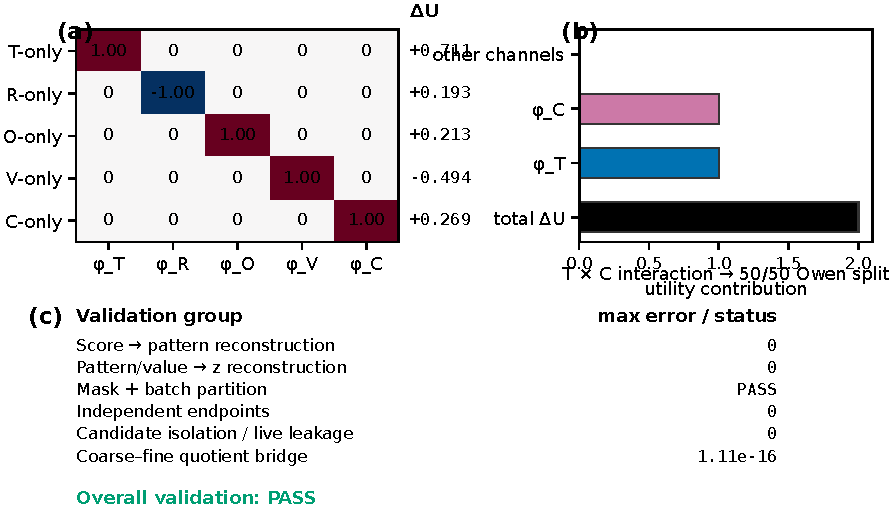
\includegraphics[width=\textwidth]{figures/Fig3.pdf}
\caption{Controlled validation of the FALI intervention semantics. (a) In five deterministic single-factor systems, attribution is isolated to the manipulated factor; the values at right give the corresponding endpoint changes. (b) A pure $T\times C$ interaction with total change approximately 2 receives the expected 1/1 Owen split between $T$ and $C$. (c) Random-transformer reconstruction, endpoint, intervention-isolation, and quotient-game checks pass, with maximum coarse--fine discrepancy $1.11\times10^{-16}$}
\label{fig:validation}
\end{figure*}


\subsection{Synthetic ground truth}\label{sec:synthetic}

We constructed deterministic attention systems containing masked softmax, values, $z=PV$, and a context-specific readout, then evaluated all 32 FALI cells. In five single-factor systems, only the manipulated factor received attribution up to floating-point precision. A separate pure $T\times C$ interaction produced the analytically expected equal Owen allocation between $T$ and $C$, with the remaining factors at zero. The all-intact and all-perturbed hybrids reconstructed their endpoints exactly at recorded precision, and collapsing $T,R,O$ into SCORE reproduced the corresponding SCORE\slash VALUE\slash CONTEXT quotient game with maximum discrepancy $1.11\times10^{-16}$.

\subsection{Transformer implementation invariants}\label{sec:implementation-validation}

We then repeated the mechanical checks in a randomly initialized two-layer TransformerLens model. Masked softmax reconstructed the cached attention patterns, pattern--value multiplication reconstructed the candidate head output, batch-specific $T/R/O$ masks formed a complete non-overlapping partition of valid scores, and candidate-output injection prevented live candidate computation from leaking into hybrid cells.

Independent ordinary forward passes gave intact effect $0.455046$, conditional effect $-0.085684$, and conditional gain $-0.540729$; the corresponding FALI endpoints reproduced all three with zero recorded discrepancy. Non-candidate heads remained unchanged under candidate-output overwrite, and the fine game agreed exactly with the collapsed coarse quotient game.

Together, these tests establish factor isolation, structural masking, endpoint recovery, intervention isolation, and coarse--fine reconciliation for the implemented pipeline. They do not establish that the factorization is unique, that hybrid states lie on the model's natural activation manifold, or that a large attribution identifies a unique natural pathway.

\paragraph{Use of generative AI tools.}
Generative AI tools, including OpenAI ChatGPT and Cursor, were used during manuscript development for literature-search support, drafting and editing, code generation and review, figure-layout development, and LaTeX/repository integration. All experimental designs, analyses, numerical results, citations, scientific claims, and final manuscript content were reviewed and verified by the authors against the underlying source code, result artifacts, and primary literature. The authors retain full responsibility for the work and its conclusions.
